% 
% Annual CCN conference
% Sample LaTeX Two-Page Summary -- Proceedings Format
% based on the prior cognitive science style file

% Original : Ashwin Ram (ashwin@cc.gatech.edu)       04/01/1994
% Modified : Johanna Moore (jmoore@cs.pitt.edu)      03/17/1995
% Modified : David Noelle (noelle@ucsd.edu)          03/15/1996
% Modified : Pat Langley (langley@cs.stanford.edu)   01/26/1997
% Latex2e corrections by Ramin Charles Nakisa        01/28/1997 
% Modified : Tina Eliassi-Rad (eliassi@cs.wisc.edu)  01/31/1998
% Modified : Trisha Yannuzzi (trisha@ircs.upenn.edu) 12/28/1999 (in process)
% Modified : Mary Ellen Foster (M.E.Foster@ed.ac.uk) 12/11/2000
% Modified : Ken Forbus                              01/23/2004
% Modified : Eli M. Silk (esilk@pitt.edu)            05/24/2005
% Modified : Niels Taatgen (taatgen@cmu.edu)        10/24/2006
% Modified : David Noelle (dnoelle@ucmerced.edu)     11/19/2014
% Modified : Konrad Kording (koerding@gmail.com) 2/15/2017

\documentclass[10pt,letterpaper]{article}

\usepackage{ccn}
\usepackage{pslatex}
\usepackage{apacite}
\usepackage{graphicx}

\title{Familiarity strengthens visual object representations}
 
\author{{\large \bf Jasper J.F. van den Bosch (vandejjf@bham.ac.uk)} \\
  A Department, 1234 Example Street\\
A City, State 12345 A country
  \AND {\large \bf Cyril Pernet (cyril.pernet@ed.ac.uk)} \\
  A Department, 1234 Example Street\\
A City, State 12345 A country
  \AND {\large \bf Ian Charest (charesti@bham.ac.uk)} \\
  A Department, 1234 Example Street\\
A City, State 12345 A country}


\begin{document}

\maketitle


\section{Abstract}
{
\bf
We are exposed to personally meaningful objects throughout the 
course of our life, and this must  be reflected in the brain. 
Despite evidence for larger brain activity, the impact of 
familiarity on the spatio-temporal dynamics of object recognition 
remains poorly understood. Here we set out to track neural 
representations of familiar and unfamiliar objects in the human 
brain as they evolve in space and time. Participants (n=20), 
saw personally-meaningful and unfamiliar objects matched in 
category and concept (72 images, including faces, bodies, 
places, objects and pets) while we recorded electroencephalography 
(EEG) and functional Magnetic Resonance Imaging (fMRI) (in separate 
sessions). Using similarity-based fusion, we combined the precise 
temporal resolution of EEG with the precise spatial resolution of 
fMRI to map the spatio-temporal trajectories of personally-meaningful 
and unfamiliar object representations. These followed the typical 
cascade of visual processes bilaterally from primary visual cortex 
(V1; ~90ms) through to the ventral and dorsal streams (~130ms). 
Critically, our results strengthen our understanding of the interactions 
between the visual sensory system, the medial temporal lobes, and 
the prefrontal cortex in recognising visual objects. 
}
\begin{quote}
\small
\textbf{Keywords:} 
familiarity; fmri; eeg; rsa
\end{quote}

\section{Introduction}

The things we see everyday vary greatly in how well we know them. 
Many lab experiments on object vision use images of things that 
the participant has not seen before. However, familiarity with 
an object has been observed to improve recognition performance, 
suggesting that it plays a key role in how we process the stimulus. 
This effect has been widely studied in faces; documenting a response 
80ms faster for familiar faces on several tasks (Ramon and Gobbini 2018, 
Visconti di Oleggio Castello et al. 2017). 
Electroencephalography (EEG) studies revealed  amplified neural 
activity in response to familiar objects (Herzmann et al. 2004). 
Functional differences between familiar and unfamiliar objects 
have also been revealed using functional Magnetic Resonance Imaging (fMRI)
\cite{Barense2011-bl,McLelland2014-es,Taylor2009-hw,Trinkler2009-dm} 
Studies increasingly turn to multivariate pattern analyses (MVPA) 
to characterise finer distinctions between experimental conditions 
from the experimental data. For example, Representational Similarity 
Analyses (RSA; Kriegeskorte et al. 2008), enables measuring fine-grained 
representational geometries in different regions of the brain, 
and testing specific hypothesis with computational or theoretical 
models (Kriegeskorte and Kievit 2013). This yielded an understanding 
of the functional properties of human inferior temporal cortex, 
with activity patterns clustering according to categories 
(Haxby et al. 2001; Kriegeskorte et al. 2008), which in turn are 
reflected in perceived similarity judgements (Mur et al. 2013).  
Linear classifiers applied to M/EEG data further revealed that 
individual object exemplars can be decoded from around 100ms 
after their presentation (Carlson et al. 2013). 

Representational geometries measured using RSA can be 
compared between measurement modalities, lending it to 
map object representations in space and time 
(Cichy et al. 2014; Cichy et al. 2016). One key aspect of 
familiarity is its idiosyncratic nature; we each have a 
different level of familiarity with a given thing. In previous work 
(Charest et al. 2014), we observed that the object representations 
in IT reflect such differences, and that these are stable across days. 
More recently, a study of face perception using RSA found that 
representations of famous celebrity faces, which have a degree of 
familiarity for all participants, are enhanced early on when 
compared to unfamiliar faces (Dobs et al. 2019). 

Here, we collected EEG and fMRI data while participants viewed 
personally meaningful or unfamiliar images, from a wide range 
of object categories including animals, bodies, faces, objects, 
and places. Using RSA, we combine data from both modalities to 
reveal the role of familiarity in object as representations 
unfold in space and time.

\begin{figure*}[t]
\begin{center}
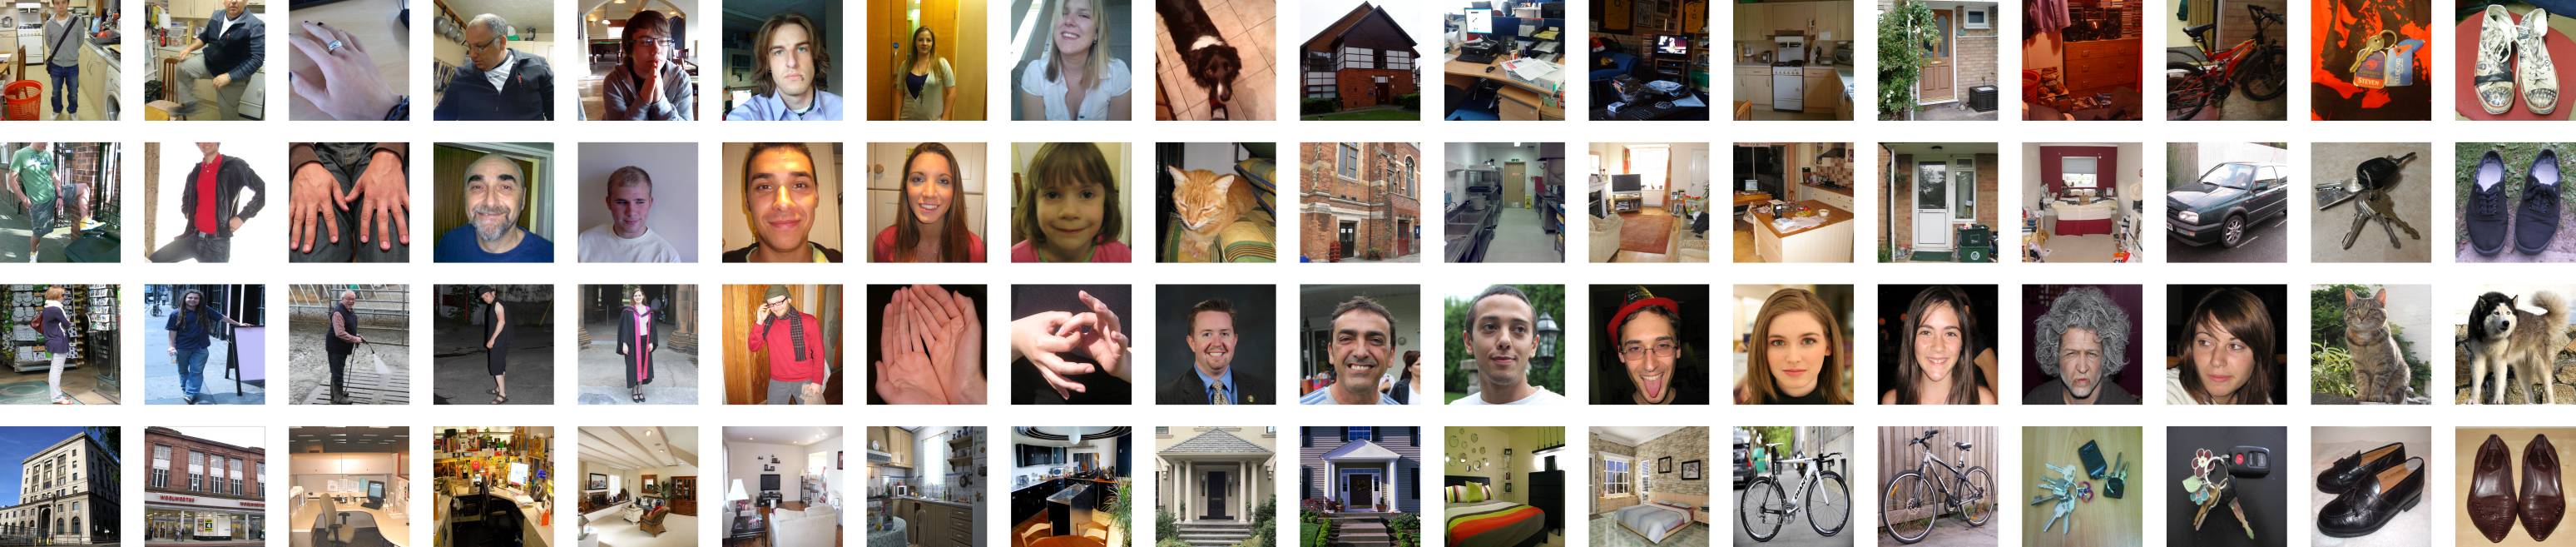
\includegraphics[width=\linewidth]{figures/figure1.png}
\end{center}
\caption{
  Stimulus materials. The first two rows depict example 
  stimuli for a pair of participant. The bottom row depicts the 
  visual object images shown to all pairs of participants.
} 
\label{fig1}
\end{figure*}

\section{Methods}

\subsection{Stimuli}

The experimental design and stimulus conditions were identical to 
(Charest et al. 2014). Briefly, participants were asked to provide 
18 images depicting objects in their daily environment (including 
faces, bodies, places, objects and pets). Participants were paired, 
and a pair of participants saw each other’s personally meaningful 
images, and a set of 36 conceptually matched images of objects from 
the same categories, shown to all participant pairs. This resulted 
in a total set of 72 stimuli (Figure~\ref{fig1}).


\subsection{Electroencephalography}

20 participants (10 female, age=23.2+-6.11) were recruited for the 
EEG. The participants had normal or corrected to normal vision, 
and no history of neurological conditions. Participants were either 
awarded course credits or a financial compensation (£7/h) for 
participating in the experiment. The experiment was approved by the 
local ethics committee at the University of Birmingham.
The EEG experiment was divided in 30 short 5 minute runs. In each run, 
the 72 stimuli were each presented once in a random order. Stimuli were 
shown for 500 ms, followed by a white fixation cross for 1500 ms (+- 
random 250ms jitter before the next trial). Every five trials, the 
participants were presented with a screen for 3 seconds that reminded 
them to blink their eyes. This helped reducing the number of blinks 
observed in the trials of interest. An additional 20% of catch trials 
were included in each run at random, with the picture of a paper clip 
being shown for 1 s, and participants had to press the keyboard key ‘m’ 
as quickly as possible when they saw the paper clip. These trials enabled 
to monitor that participants were paying attention to the task and were 
later discarded from further analyses. EEG recordings were collected 
using a high-density EEG system (128 channel BIOSEMI active system, 
with an additional 3 electrodes positioned on the two mastoids and 
beneath the participant’s dominant eye) at a sampling frequency of 
1024Hz. Condition trials were epoched from -.5s to 1.5s relative to 
stimulus onset.  Baseline correction was applied to each trial using 
a time-window centered between -.5s and the stimulus onset). This 
resulted in 30 epoched trials for each of the 72 conditions per participant.

\subsection{functional Magnetic Resonance Imaging}

20 participants (10 female, age=22.3+-4.12) were recruited from the 
Medical Research Council participant panel. Participants were provided 
with a financial compensation of £7/hour for their participation. The 
participants had normal or corrected to normal vision, no history of 
neurological conditions, and were screened for suitability for fMRI 
scanning. The experiment was approved by the Cambridge Psychology 
Research Ethics Committee. Results from this same data set have been 
published previously (Charest et al. 2014).

Noteworthy, our EEG and fMRI participants came from two independent 
samples.  The fMRI experiment has been described previously 
(Charest et al. 2014). Participants were presented with the 
stimuli and were asked to indicate on each trial whether the 
image presented had their or global details altered by pressing 
a button placed underneath their middle finger. If the image was 
the original image (no alterations), participants pressed a button 
placed underneath their index finger.  

fMRI volumes were first converted to DICOM, and organised using the 
Brain Imaging Data Standards (BIDS, Gorgolewski et al. 2016). The 
BIDS dataset was then pre-processed using fMRI-prep (Esteban et al. 2019). 
EPI images were slice-time corrected, corrected for spatial alignment, 
and normalised to the Montreal Neurological Institute ICBM template 
space (Mazziotta et al. 2001). After this initial pre-processing, we 
used GLMdenoise (Kay et al. 2013; Charest et al. 2018) to fit the 
EPI data. 

\subsection{Representational Similarity Analysis}

To characterise the temporal dynamics of the brain representational 
geometries, we used representational dissimilarity matrices (RDMs) 
constructed from each time point of the EEG data. We used a linear 
discriminant analysis for each pair of stimuli at each time point 
using MVPA-Light (http://www.github.com/trederm/MVPA-Light) in 
Matlab (The MathWorks, Natinck, USA). The features provided to 
the LDA were the 128 electrode activity patterns for a given time 
point. Importantly the LDA analysis was performed using a stratified 
k-fold cross-validation scheme (5-fold cross-validation, 5 repetitions) 
applied to out of sample test data, preventing from overfitting. For 
each pair, the averaged cross-validated decoding accuracy was used 
as a proxy for that pair’s distance in a representational space.

The fMRI beta estimates provided by GLMdenoise were normalised 
using a univariate normalisation (Misaki et al. 2010) before 
entering an RSA searchlight analyses. The RSA searchlight analysis 
was performed using pyRSA ( https://github.com/Charestlab/pyrsa ).  
The fMRI volumes were segmented in 6mm diameter spheres centred 
on every voxel contained inside the participant’s brain. For each 
sphere, we extracted the 72 t-patterns (one t-pattern per visual 
condition) indexed by the voxels of the sphere. From these voxel 
t-patterns, we constructed RDMs using a Pearson correlation distance, 
and this RDM was assigned to the voxel at the center of the 
searchlight sphere. The Pearson correlation distance applied on 
univariate normalised GLMdenoised beta estimates was chosen after 
having previously shown to be the most reliable measure of 
representational geometries (Charest et al. 2018). 


\section{Acknowledgments}

This work was supported by an European Research Council (ERC) 
Starting Grant ERC-2017-StG 759432 (to I.C.)


\bibliographystyle{apacite}

\setlength{\bibleftmargin}{.125in}
\setlength{\bibindent}{-\bibleftmargin}

\bibliography{vandenbosch}


\end{document}
